\section{Controlpath}
The control path is not designed as a finite state machine. Due to its simplicity we chose an approach that is closer to the pipelined structure of the MIPS-Architecture. The control path is built around a 32-bit wide 4-deep shift register. When the memory returns the instruction to the instruction-decode-stage of the datapath, it is also fed into the shift register and propagates in the following clock cycles. To the stages of this shift register we attatched a decoder that produces control signals for one stage of our datapath. Each stage of the shift register matches exactly one stage of the datapath, except for the first controller stage which handles instruction fetch and instruction decode. The second stage returns the control signals for the execution stage, the third stage is mapped to the memory stage and the fourth stage controls the datapath's writeback stage. In case of any stalls the propagation of the instructions through the shift register is halted.
\begin{figure}[h!]
  \centering
  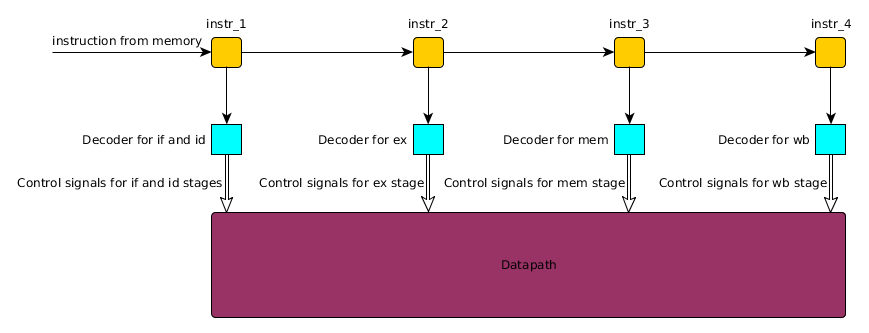
\includegraphics[width=1.0\textwidth]{figure/control.png}
  \caption{Control path}
  \label{fig:control}
\end{figure}
\subsection{Decoder for the instruction-fetch- and instruction-decode-stage}
The decoder attatched to the first stage of the shift register distinguishes between the opcodes of the given instruction to determine the control signals. If the opcode is 000000, an R-type-instruction is assumed and the instruction-decode-stage's destination register control signal is set to 0 to use the R-type destination register. The shift multiplexor is set to 0 as well to use the R-type-instructions shift field. For the settings of the pc's multiplexor in the instruction-fetch-stage, the other bits of the instruction are evaluated. If they make the instruction a Jump-Register-instruction, the signal is set to 1 so that the new program counter calculated by the branch logic is used instead of the previous value incremented by 4. In every other case, this multiplexor's control signal is set to zero because all other R-type-instructions do not modify the program counter.\\
All non-R-type-instructions are treated as I-type-instructions by the decoder. This means, that the control signal for the shift-multiplexor is set to 0 for all instructions except the LUI-Instruction, which needs a shift of 16. Therefore, the signal is set to 1. A more complex decision has to be made for the program counter multiplexor. All instructions that influence the program's control flow (Branch- and Jump-Instructions) produce an output of 1, all other instructions return 0 and the program counter is incremented by 4. The multiplexor for the destination register is always set to 2 to use the I-type-instruction destination field. This is again ignored, when a J-type-instruction reaches the further stages, so no damage is done.
\subsection{Decoder for the execution-stage}
The decoder for the execution stage has to set the signals that select the operands of the operation to be executed and set the kind of operation the ALU has to perform. Since the instruction's opcode is in hardly any way connected to the executed operation, the decoder logic is a little more difficult. It groups all operations of the example code that perform an addition of a register's value to the immediate value of the instruction (ADDIU, LW, SW, SB, LBU) and sets the control signals to 2 for the ALU's a-operand, 1 to forward the immediate field to the ALU and the ALU's operation code itself is set to 20 for addition. For the LUI-instruction, the ALU's a-operand-multiplexor is set to 0 for a shift of 16, the b-operand-multiplexor is set to 1 for the immediate-field and the ALU itself is perfoming the shift operation. All other immediate-operations get the a-operand-multiplexor set to 2, b set to 1 and the ALU operation code set according to the instruction. The only supported R-type operation, SLT gets a set to 2, b set to 0 and the ALU set for set-less-than-operations. All other R-Type instructions are treated like NOOP-instructions: A set to 2, b set to 0 and the ALU-operation set to a left-shift. Although the datapath would be able to support more operations, the datapath is limited to the described instructions and has to be expanded for a full MIPS instruction set.
\subsection{Decoder for the memory stage}
The memory stage's decoder is more simple than the execution stage's decoder. It just has to evaluate whether the instruction is a store-instruction, a load-instruction or any other instruction. In case of a load instruction the multiplexor signal for the memory access has to be set to 1 to let the result of the memory access get to the writeback stage. In all other cases, this signal is set to 0 to just forward the signal coming from the execution stage. The read or write masks are set according to the instruction stored in the shift register stage. A SW-instruction for example produces an output of F for the write mask and an LBU-instruction returns a read mask of 1. All other instructions have read and write masks of 0.
\subsection{Decoder for the writeback stage}
The decoder for the writeback stage is the simplest of the whole controller because it controls just one signal that enables the register bank. It distinguishes between the commands that write back to the register bank bank (currently supported: LUI, ADDIU, LW, LBU, SLTI, SLT, ANDI, ORI) and sets the \em enable\_ regs\em -signal to for them, and the other instructions, where the register bank is disabled by setting the signal to zero. 